\chapter{植被生物地球化学循环过程}\label{植被生物地球化学循环过程}
%\addcontentsline{toc}{chapter}{植被生物地球化学循环过程}

%\begin{植被生物地球化学循环过程}
CoLM植被生物地球化学循环模块存在复杂的碳氮循环网络,植物生理和物候等过程是量化不同碳氮库相互转换和传输的关键。
光合作用是植被生物地球化学循环的初始输入。光合作用的碳输入扣除植被的自养呼吸得到净初级生产力将被分配到植被不同营养器官中,
植被的自养呼吸和碳氮分配是其中的关键过程。同时,植被生长存在季节变化特征,特别是落叶植被功能型,
物候过程影响植被生物地球化学循环的季节性模拟。物候过程同样模拟叶和细根的凋落过程,
植被碳氮库的周转由物候过程和植被自然死亡过程共同控制。
经过物候过程和植被自然死亡过程,植被凋落物进入土壤进一步进行地下生物地球化学循环。
\section{植被自养呼吸}\label{植被自养呼吸}
CoLM的自养呼吸$CF_{ar,total}$计算包括维持呼吸$CF_{mr,total}$和生长呼吸$CF_{gr,total}$,
模型对他们分别进行模拟 \citep{lavigne1997growth,sprugel1995respiration}。
自养呼吸指植被活体组织维持正常的代谢活动所消耗的碳,生长呼吸指植被生长所消耗的碳。
\begin{equation}
CF_{ar,total}=CF_{mr, total}+CF_{gr,total}
\end{equation}
\subsection{维持呼吸}
叶片的维持呼吸($R_d$)由光合作用模块中公式(\ref{R_d1})计算。
除此之外,活茎、活粗根和细根同样存在维持呼吸。
维持呼吸和植被器官单位面积的氮含量成正比,同时受到温度的调控:
\begin{equation}
CF_{{livestem}}=N_{{livestem }} \cdot R_{{base }} \cdot R_{q10}^{\left(T_{2m}-20\right) / 10}
\end{equation}
\begin{equation}
CF_{ {livecroot }}=N_{ {livecroot }} \cdot R_{ {base }} \cdot R_{q10}^{\left(T_{2m}-20\right) / 10}
\end{equation}
\begin{equation}
CF_{ {froot }}=N_{{froot}} \cdot R_{{base}} \cdot R_{q10}^{\left(T_{2m}-20\right) / 10}
\end{equation}
其中$CF_{livestem}$,$CF_{livecroot}$和$CF_{froot}$分别是活茎、活粗根和细根的维持呼吸速率。
$R_{q10}$是维持呼吸的温度敏感性参数,$T_{2m}$是2m高度气温, $N_{livestem}$,$N_{livecroot}$和$N_{froot}$
分别代表单位面积活茎氮含量、活粗根氮含量和活细根氮含量。$R_{base}$是基础维持呼吸速率。
木本植物功能型存在死茎和死粗根库,但维持呼吸的计算不包括死茎和死粗根库。因此,假设基础维持呼吸速率为常数。
总维持呼吸$CF_{mr,total}$的计算包括叶、活茎、活粗根和细根的维持呼吸的总和:
\begin{equation}
CF_{mr,total}=R_{d}+CF_{livestem}+CF_{livecroot}+CF_{froot}
\end{equation}
\subsection{生长呼吸}\label{生长呼吸}
生长呼吸$CF_{gr,total}$由植被单位面积的净生长速率乘以系数0.11得到:
\begin{equation}
CF_{gr,total}=NPP \cdot 0.11
\end{equation}
植被单位面积单位时间的净生长速率由净初级生产力($NPP$)来代表,$NPP$是光合作用速率和自养呼吸速率的差值,
并且同时考虑了土壤的氮限制,其详细计算见章节 \ref{植被土壤的氮竞争} 植被土壤的氮竞争。生长呼吸的计算方案是基于\citet{atkins2018quantifying}
的通量站点的木质和非木质组织的构造消耗研究得出的。在模型中,假设生长呼吸发生时间与碳分配的发生同步。
\section{植被碳氮分配}\label{植被碳氮分配}
\subsection{维持呼吸的碳消耗}
CoLM碳分配首先满足维持呼吸($CF_{mr,total}$)的需求,其次碳分配需要填补由于夜间或冬天光合作用少于维持呼吸所造成的碳存储亏缺,
最后剩余碳分配才能用于植被各营养器官库的生长。所以由光合作用支持的维持呼吸碳供给($CF_{GPP,mr}$)可以表达为:
\begin{equation}\label{F_GPP_mr}
CF_{GPP,mr}=\left\{\begin{array}{cl}CF_{mr, total} & \text{当}\quad CF_{mr, total} \leq CF_{GPP} \\ CF_{GPP} & \text{当}\quad CF_{mr,total}>CF_{GPP} \end{array}\right.
\end{equation}
其中,$CF_{GPP}$代表实际光合作用碳收入,正常情况,$CF_{GPP}\geq CF_{mr,total}$,
维持呼吸的消耗($CF_{mr,total}$)可以完全由光合作用($CF_{GPP}$)提供。
但夜间和冬天光合作用的碳收入通常会低于呼吸作用的碳消耗,维持呼吸仅部分由光合作用支持,另外一部分($CF_{xs,mr}$)由植被呼吸碳储存库($CS_{xs}$)支持:
\begin{equation}\label{CF_xs_mr}
CF_{xs, mr}=\left\{\begin{array}{cl}0 & \text{当}\quad CF_{mr, total} \leq CF_{GPP} \\ CF_{mr, total}-CF_{GPP} & \text{当}\quad CF_{mr, total}>CF_{GPP}\end{array}\right.
\end{equation}
联合公式(\ref{F_GPP_mr})和(\ref{CF_xs_mr}),可以保证维持呼吸的碳平衡关系:
\begin{equation}
CF_{GPP, mr}+CF_{xs, mr}=CF_{mr, total}
\end{equation}


\subsection{用于植被呼吸的碳储存库}
植被呼吸的碳储存库($CS_{xs}$)会根据光合作用对维持呼吸的亏缺和补充进行更新,其每个时间步长的变化量($\Delta CS_{xs}$)可表示为:
\begin{equation}
\Delta CS_{xs}=\left(CF_{GPP, xs}-CF_{xs, mr}\right) \cdot \Delta t
\end{equation}
$\Delta t$代表模型时间步长,$CF_{GPP,xs}$是光合作用对植被的呼吸碳储存库($CS_{xs}$)的补充。

由于光合作用对维持呼吸存在亏缺的可能性,植被的呼吸碳储存库($CS_{xs}$)也存在负值。
光合作用对植被呼吸碳存储库($CS_{xs}$)的补充($CF_{GPP,xs}$)仅当该库为负值时存在,并且须首先满足维持呼吸的需要。
\begin{equation}
CF_{GPP, xs}=\left\{\begin{array}{ll}0 & CS_{xs} \geq 0 \\ \min \left(-\frac{CS_{xs}}{86400 \cdot \tau_{xs}}, \max \left(CF_{GPP}-CF_{GPP, mr}, 0\right)\right) & CS_{xs}<0\end{array}\right.
\end{equation}
其中$\tau_{xs}=30$天,$-\frac{CS_{xs}}{86400 \tau_{xs}}$代表如果光合作用碳收入充足,最快需要30天将亏缺的植被呼吸碳存储库($CS_{xs}$)填补上。
当然,如果扣除维持呼吸后的碳收入不足以维持$-\frac{CS_{xs}}{86400 \tau_{xs}}$,其补充的碳通量为光合作用扣除维持呼吸后的剩余碳收入,
即$\max{\left(CF_{GPP}-CF_{GPP,mr},0\right)}$。


\subsection{植被的碳氮生长分配比例}
用于植被生长的碳收入,即可分配碳($CF_{avail\_alloc}$),是光合作用碳通量($CF_{GPP}$)扣除维持呼吸($CF_{GPP,mr}$)和对植被呼吸碳存储的补充($CF_{GPP,xs}$)后的剩余碳收入:
\begin{equation}
CF_{ {avail\_alloc }}=CF_{GPP}-CF_{GPP, mr}-CF_{GPP, xs}
\end{equation}
植物各器官所分配到的碳的比例由分配系数参数决定:
\begin{enumerate}
  \item 新生长细根和新生长叶的比例$a_1$; 
  \item 新生长活粗根和新生长活茎的比例 $a_2$;
  \item 新生长活茎和新生长叶的比例$a_3$;
  \item 新生长活茎和新生长叶的比例$a_3$;
  \item 新生长活茎在新生长总茎(活茎+死茎)碳含量的比例$a_4$;
  \item 生长呼吸在总生长碳的比例 $g_1$,这些分配系数参数取决于其所属植被功能型。其中,新生长活茎和新生长叶的比例$a_3$由前一年的年$NPP_{ann}$ ($\mathrm{g\ C\ m^{-2}\ year^{-1}}$)决定:
    \begin{equation}
      a_{3}=\frac{2.7}{1+e^{-0.004 \cdot\left(NPP_{ann}^{-300}\right)}}-0.4
    \end{equation}
\end{enumerate}

因此,随着$NPP$增加,植被倾向于将更多的碳分配给茎 \citep{allen2005,vanninen2005carbon}。
因此叶片的单位碳生长需要植被的总碳输入是:
\begin{equation}\label{C_allom}
C_{ {allom }}=\left\{\begin{array}{lr}\left(1+g_{l}\right)\left[1+a_{1}+a_{3}\left(1+a_{2}\right)\right] &  \text{ woody } \text{PFT} \\ 
  \left(1+g_{l}\right)\left(1+a_{1}\right) &  \text{ non }- \text{ woody } \text{PFT}\end{array}\right.
\end{equation}
植被氮分配与碳分配共享同样一套分配系数参数,结合各器官的碳氮比参数,叶片的单位碳生长需要植被的总氮输入是:
\begin{equation}\label{N_allom}
N_{ {allom }}= \begin{cases}
\frac{1}{CN_{ {leaf }}}+\frac{a_{1}}{CN_{ {froot }}}+\frac{a_{3} a_{4}\left(1+a_{2}\right)}
  {CN_{l w}}+\frac{a_{3}\left(1-a_{4}\right)\left(1+a_{2}\right)}{CN_{d w}}  &  \text { woody PFT} \\ 
  \frac{1}{CN_{ {leaf }}}+\frac{a_{1}}{CN_{ {froot }}} & \text { non--woody PFT}
  \end{cases}
 \end{equation}
$CN_{leaf}$,$CN_{froot}$,$CN_{lw}$ 和 $CN_{dw}$ 分别代表叶、细根、活木和死木的碳氮比。
根据植被可分配碳($CF_{avail\_{alloc}}$),可以算出植被的氮需求($NF_{plant\_{demand}}$):
\begin{equation}
N F_{ {plant\_{demand }}}=CF_{ {avail\_{alloc }}} \cdot \frac{N_{ {allom }}}{C_{ {allom }}}
\end{equation}
然而,实际碳生长($CF_{actual\_{alloc}}$)需要根据实际的氮供给($NF_{actual\_{alloc}}$)来计算。
实际氮供给($NF_{actual\_{alloc}}$)来源于植被氮重利用($NF_{retran\_{alloc}}$)和土壤无机氮摄取($NF_{sminn\_{alloc}}$)两部分:
\begin{equation}\label{NF_actual_alloc}
NF_{actual\_{alloc}}=NF_{retran\_{alloc}}+NF_{sminn\_{alloc}}
\end{equation}


\subsection{植被氮重利用}\label{植被氮重利用}
植被营养器官在凋落前通常会回收部分氮以用于新组织的生长,
被称为植被氮的重利用 \citep{magill1997biogeochemical,oikawa2005dynamics,son1991aboveground}。
植被氮重利用的计算依赖于植被氮重利用库($NS_{retrans}$)和植被氮需求($NF_{plant\_{demand}}$)。
其中,可用于生长的重利用氮($NF_{avail\_{retran}}$)与植被氮需求($NF_{plant\_{demand}}$)成正比:
\begin{equation}
NF_{avail\_retrans}=\min{\left(\frac{NF_{retrans\_ann}\ \cdot \frac{NF_{plant\_demand}}{NF_{plant\_demand\_ann}}}{{\Delta t}}, \frac{NS_{retrans}}{{\Delta t}}\right)}
\end{equation}
其中,$NF_{retrans\_ann}$是去年植被重利用氮总量 ($\mathrm{g\ N\ m^{-2}\ year^{-1}}$),$NF_{plant\_demand\_ann}$ 是去年植被氮需求总量 ($\mathrm{g\ N\ m^{-2}\ year^{-1}}$),${\Delta t}$ 是模型的时间步长。
实际来源于重利用氮库的氮通量 ($NF_{retran\_alloc}$) 是可利用氮 ($NF_{avail\_retrans}$) 和氮需求 ($NF_{plant\_demand}$) 的最小值:
\begin{equation}\label{NF_retran_alloc}
  NF_{retran\_alloc}=\min{\left(NF_{avail\_retrans}, NF_{plant\_demand}\right)}
\end{equation}


\subsection{土壤无机氮摄取}\label{土壤无机氮摄取}
由于植被氮的重利用,植被对土壤的无机氮需求 ($NF_{plant\_demand\_soil}$) 降低为:
\begin{equation}\label{NF_plant_demand_soil}
  NF_{plant\_demand\_soil} = NF_{plant\_demand} - NF_{retran\_alloc}	       
\end{equation}
由于不同植被功能型对于有限的土壤无机氮的竞争,以及土壤微生物和植被之间的竞争,植被从土壤中的无机氮摄取将进一步缩减:
\begin{equation}\label{NF_sminn_alloc}
NF_{sminn\_alloc} = NF_{plant\_demand\_soil}\cdot f_{plant\_demand}
\end{equation}
其中,$f_{plant\_demand}$ 是植被氮摄取的限制因子,其范围在0到1之间。其具体计算将在章节~\ref{植被土壤的氮竞争} 植被土壤的氮竞争中介绍。


\subsection{植被的碳氮生长分配}\label{植被的碳氮生长分配}
通过公式 \eqref{NF_sminn_alloc}, \eqref{NF_retran_alloc} 和 \eqref{NF_actual_alloc},实际氮供给 ($NF_{actual\_alloc}$) 可以被模型计算,
再联立公式 \eqref{C_allom} 和 \eqref{N_allom},实际植被碳生长 ($CF_{actual\_alloc}$) 可以被计算:
\begin{equation}
  CF_{actual\_alloc} = NF_{actual\_alloc}\frac{C_{allom}}{N_{allom}}
\end{equation}
同时,容易计算叶碳的实际生长:
\begin{equation}
  CF_{alloc\_leaf\_total} = CF_{actual\_alloc}/C_{allom}
\end{equation}
假设碳分配到组织碳库和非结构碳库的比例固定 $\left(f_{cur}:\left(1-f_{cur}\right)\right)$,
$f_{cur}$为新生长的组织库所占的比例。根据分配系数参数,各个器官的碳生长可以被计算:
\begin{equation}\label{CF_alloc_{leaf}}
  CF_{alloc,leaf} = CF_{alloc_{leaf\_total}}\cdot  f_{cur}
\end{equation}
\begin{equation}
  CF_{alloc,leaf\_storage} = CF_{alloc\_leaf\_total}\cdot \left(1-f_{cur}\right)
\end{equation}
\begin{equation}
  CF_{alloc,froot} = CF_{alloc_{leaf\_total}}\cdot a_1\cdot f_{cur}
\end{equation}
\begin{equation}
  CF_{alloc,{froot\_storage}} = CF_{alloc\_leaf\_total}\cdot a_1\cdot \left(1-f_{cur}\right)
\end{equation}
如果是木本植物类型,碳分配器官还包括茎和粗根:
\begin{equation}
  CF_{alloc,livestem} = CF_{alloc\_leaf\_total}\cdot a_3a_4\cdot f_{cur}
\end{equation}
\begin{equation}
  CF_{alloc,livestem\_storage} = CF_{alloc\_leaf\_total}\cdot a_3a_4\cdot \left(1-f_{cur}\right)
\end{equation}
\begin{equation}
  CF_{alloc,deadstem} = CF_{alloc\_leaf\_total}\cdot a_3\left(1-a_4\right)\cdot f_{cur}
\end{equation}
\begin{equation}
  CF_{alloc,deadstem\_storage} = CF_{alloc\_leaf\_total}\cdot a_3\left(1-a_4\right)\cdot \left(1-f_{cur}\right)
\end{equation}
\begin{equation}
  CF_{alloc,livecroot} = CF_{alloc\_leaf\_total}\cdot a_2a_3a_4\cdot f_{cur}
\end{equation}
\begin{equation}
  CF_{alloc,livecroot\_storage} = CF_{alloc\_leaf\_total}\cdot a_2a_3a_4\cdot \left(1-f_{cur}\right)
\end{equation}
\begin{equation}
  CF_{alloc,deadcroot} = CF_{alloc\_leaf\_total}\cdot a_2a_3\cdot \left(1-a_4\right)\cdot f_{cur}
\end{equation}
\begin{equation}\label{CF_alloc_deadcroot_{storage}}
  CF_{alloc,deadcroot\_storage} = CF_{alloc\_leaf\_total}\cdot a_2a_3\left(1-a_4\right)\cdot \left(1-f_{cur}\right)
\end{equation}
将公式 \eqref{CF_alloc_{leaf}}--\eqref{CF_alloc_deadcroot_{storage}} 求和可得,因此碳平衡得以保证:
\begin{equation}
  \sum_{i}{CF_{alloc,i}}=CF_{actuall\_alloc}
\end{equation}
其中 $CF_{alloc,i}$ 代表每个植被库的新生长碳含量,
$i$等于$leaf$、$leaf\_storage$、$froot$、$froot\_storage$、$livestem$、$livestem\_storage$、$deadstem$、
 $deadsteam\_storage$、$livecroot$、 $livecroot\_storage$、$deadcroot$
 和 $deadcroot\_storage$ 分别代表叶库、叶存储库、细根库、细根存储库、活茎库、
 活茎存储库、死茎库、死茎存储库、活粗根库、活粗根存储库、死粗根库和死粗根存储库的新生长碳含量。


 对应各个器官的氮生长也可以计算:
\begin{equation}\label{eq:NF_alloc_leaf}
  NF_{alloc,leaf} = \frac{CF_{alloc\_leaf_total}}{CN_{leaf}}\cdot f_{cur}
\end{equation}
\begin{equation}
  NF_{alloc,leaf\_storage} = \frac{CF_{alloc\_leaf\_total}}{CN_{leaf}}\cdot \left(1-f_{cur}\right)
\end{equation}
\begin{equation}
  NF_{alloc,froot} = CF_{alloc\_leaf\_total}\cdot \frac{a_1}{CN_{froot}}\cdot f_{cur}
\end{equation}
\begin{equation}
  NF_{alloc,froot\_storage} = CF_{alloc\_leaf\_total}\cdot \frac{a_1}{CN_{froot}}\cdot \left(1-f_{cur}\right)
\end{equation}

如果是木本植物类型,碳分配器官还包括茎和粗根:
\begin{equation}
  NF_{alloc,livestem} = CF_{alloc\_leaf\_total}\cdot \frac{a_3a_4}{CN_{lw}}\cdot f_{cur}
\end{equation}
\begin{equation}
  NF_{alloc,livestem\_storage} = CF_{alloc\_leaf\_total}\cdot \frac{a_3a_4}{CN_{lw}}\cdot \left(1-f_{cur}\right)
\end{equation}
\begin{equation}
  NF_{alloc,deadstem} = CF_{alloc\_leaf\_total}\cdot \frac{a_3\left(1-a_4\right)}{CN_{dw}}\cdot f_{cur}
\end{equation}
\begin{equation}
  NF_{alloc,deadstem\_storage} = CF_{alloc\_leaf\_total}\cdot \frac{a_3\left(1-a_4\right)}{CN_{dw}}\cdot \left(1-f_{cur}\right)
\end{equation}
\begin{equation}
  NF_{alloc,livecroot} = CF_{alloc\_leaf\_total}\cdot \frac{a_2a_3a_4}{CN_{lw}}\cdot f_{cur}
\end{equation}
\begin{equation}
  NF_{alloc,livecroot\_storage} = CF_{alloc\_leaf\_total}\cdot \frac{a_2a_3a_4}{CN_{lw}}\cdot \left(1-f_{cur}\right)
\end{equation}
\begin{equation}
  NF_{alloc,deadcroot} = CF_{alloc\_leaf\_total}\cdot \frac{a_2a_3\left(1-a_4\right)}{CN_{dw}}\cdot f_{cur}
\end{equation}
\begin{equation}\label{eq:NF_alloc_deadcroot_storage}
  NF_{alloc,deadcroot\_storage} = CF_{alloc\_leaf\_total}\cdot \frac{a_2a_3\left(1-a_4\right)}{CN_{dw}}\cdot \left(1-f_{cur}\right)
\end{equation}
将公式 \eqref{eq:NF_alloc_leaf}--\eqref{eq:NF_alloc_deadcroot_storage} 求和可得,因此氮平衡得以保证:
\begin{equation}
  \sum_{i}{NF_{alloc,i}}=CF_{actuall,alloc}\cdot \frac{N_{allom}}{C_{allom}}=NF_{actuall\_alloc}
\end{equation}
其中$NF_{alloc,i}$代表每个植被库的新生长氮含量, 
$i$ 等于 $leaf$,$leaf\_storage$,$froot$,$froot\_storage$,$livestem$,$livestem\_storage$,
$deadstem$,$deadsteam\_storage$,$livecroot$,$livecroot\_storage$,$deadcroot$,
 和 $deadcroot\_storage$ 分别代表叶库、叶存储库、细根库、细根存储库、活茎库、
 活茎存储库、死茎库、死茎存储库、活粗根库、活粗根存储库、死粗根库和死粗根存储库的新生长氮含量。


\section{植被物候过程的耦合预报方案}\label{植被物候过程的耦合预报方案}
CoLM植被物候过程的耦合预报方案通过对叶片碳的收支控制,模拟叶面积指数的季节变化特征。


\subsection{模型中的基本物候变量和概念}\label{模型中的基本物候变量和概念}

\begin{enumerate}
\renewcommand{\theenumi}{\alph{enumi}}
\item 发芽展叶期\\
CoLM物候过程模块假设落叶植被功能型存在发芽展叶期,即叶面积指数伴随着叶碳库在10多天的发芽展叶期内逐渐增加。发芽初期,非结构存储库将其一半的碳存储转给碳传输库,
在随后10多天时间里,碳传输库逐渐将碳转移给组织库,以模拟叶碳含量在此期间逐渐升高的发芽现象。模拟上通过控制从传输库$CS_{i_{xfer}}$
到组织库$CS_i$的碳转移通量$CF_{i\_xfer\rightarrow i}$来实现
($i$ 等于$leaf$,$froot$,$livestem$,$deadstem$,$livecroot$ 和
$deadcroot$ 分别代表叶、细根、活茎、死茎、活粗根和死粗根):
\begin{equation}
  CF_{leaf\_xfer\rightarrow leaf} = r_{{xfer}\_{on}}\cdot CS_{leaf\_{xfer}}\ 
\end{equation}
\begin{equation}
  CF_{froot\_{xfer}\rightarrow froot} = r_{{xfer}\_{on}}\cdot CS_{froot\_{xfer}}\ 
\end{equation}
\begin{equation}
  CF_{livestem\_{xfer}\rightarrow leaf} = r_{{xfer}\_{on}}\cdot CS_{livestem\_{xfer}}\ 
\end{equation}
\begin{equation}
  CF_{deadstem\_{xfer}\rightarrow froot} = r_{{xfer}\_{on}}\cdot CS_{deadstem\_{xfer}}\ 
\end{equation}
\begin{equation}
  CF_{livecroot\_{xfer}\rightarrow leaf} = r_{{xfer}\_{on}}\cdot CS_{livecroot\_{xfer}}\ 
\end{equation}
\begin{equation}
  CF_{deadcroot\_{xfer}\rightarrow froot} = r_{{xfer}\_{on}}\cdot CS_{deadcroot\_{xfer}}\ 
\end{equation}
在碳转移的同时,也伴随着氮转移通量($NF_{i\_{xfer}\rightarrow i}$),控制从氮传输库 $NS_{i\_{xfer}}$ 到氮组织库 $NS_{i}$ 的转移:
\begin{equation}
  NF_{leaf\_{xfer}\rightarrow leaf} = r_{{xfer}\_{on}}\cdot NS_{leaf\_{xfer}}\ 
\end{equation}
\begin{equation}
  NF_{froot\_{xfer}\rightarrow froot} = r_{{xfer}\_{on}}\cdot NS_{froot\_{xfer}}\ 
\end{equation}
\begin{equation}
  NF_{livestem\_{xfer}\rightarrow leaf} = r_{{xfer}\_{on}}\cdot NS_{livestem\_{xfer}}\ 
\end{equation}
\begin{equation}
  NF_{deadstem\_{xfer}\rightarrow froot} = r_{{xfer}\_{on}}\cdot NS_{deadstem\_{xfer}}\ 
\end{equation}
\begin{equation}
  NF_{livecroot\_{xfer}\rightarrow leaf} = r_{{xfer}\_{on}}\cdot NS_{livecroot\_{xfer}}\ 
\end{equation}
\begin{equation}
  NF_{deadcroot\_{xfer}\rightarrow froot} = r_{{xfer}\_{on}}\cdot NS_{deadcroot\_{xfer}}\ 
\end{equation}
其中,$r_{{xfer}\_{on}}$ 是控制传输库碳转移到组织库速率的变量 ($\mathrm{s^{-1}}$),是随时间变化的变量。
\begin{equation}
r_{xfer\_{on}}=\left\{\begin{array}{ll}\frac{2}{t_{ {onset}}} &  \text{ 当 }  t_{ {onset}} \neq \Delta t \\ 
\frac{1}{\Delta t} &  \text{ 当 }  t_{onset}=\Delta t\end{array}\right.
\end{equation}
$t_{onset}$以倒计时的形式记录发芽展叶期还剩多少秒,$\Delta t$是模型时间步长$t_{onset}\neq\Delta t$时,
$\frac{2}{t_{onset}}$随着时间的推移转移速率,
即叶片生长速率逐渐加快;$t_{onset}=\Delta t$时为发芽展叶期最后一个时间步长,所有传输库都将转移给组织库。\\

\item 落叶期 \\
CoLM物候模块同样假设落叶植被功能型存在落叶期,在落叶期内,叶碳库和细根碳库在为期10多天时间里逐渐降为0:
\begin{equation}
CF_{ {leaf,litter }}^{n}=\left\{\begin{array}{ll}CF_{ {leaf,litter }}^{n-1}+r_{xfer\_{off}}\left(CS_{ {leaf }}-CF_{ {leaf }}^{n-1} t_{ {offset }}\right) & \text{ 当 }  t_{ {offset }} \neq \Delta t \\ 
\frac{CS_{ {leaf }}}{\Delta t}+CF_{ {alloc,leaf }} &  \text{ 当 }  t_{offset}=\Delta t
\end{array}\right.
\end{equation}
\begin{equation}
CF_{ {froot },  { litter }}^{n}=\left\{\begin{array}{ll}CF_{ {froot }, litter}^{n-1}+r_{xfer\_off}\left(CS_{ {froot }}-CF_{ {froot }}^{n-1} t_{offset}\right) &  \text{ 当 }  t_{offset} \neq \Delta t \\ 
\frac{CS_{ {froot }}}{\Delta t}+CF_{ {alloc,froot }} &  \text{ 当 }  t_{offset}=\Delta t
\end{array}\right.
\end{equation}
\begin{equation}
r_{xfer\_off}=\frac{2 \Delta t}{t_{offset}^{2}}
\end{equation}
其中 $CF_{leaf,litter}^{n-1}$ 和 $CF_{leaf,litter}^n$ 分别代表上一个模拟时间步长和这一个时间步长的叶碳凋落通量。
$CF_{froot,litter}^{n-1}$ 和 $CF_{froot,litter}^n$ 分别代表上一个模拟时间步长和这一个时间步长的细根碳凋落通量。
$t_{offset}$ 以倒计时的形式记录落叶期还剩多少秒。$CS_{leaf}$和$CS_{froot}$代表组织库的叶碳和细根碳含量,将随着落叶期的推进逐渐下降。
另外,落叶期的凋落速率参数($r_{{xfer}\_{off}}$)将随时间逐渐增加。$t_{offset}=\Delta t$ 时为落叶期最后一个时间步长,
所有叶和细根组织库内的所有碳氮都将凋落。

叶氮和细根氮库在落叶期的凋落通量($NF_{leaf,litter}$ 和 $NF_{froot,litter}$)
还与叶和根的碳氮比 ($CN_{leaf}$ 和 $CN_{froot}$) 息息相关。同时,
离开叶库的氮将有一部分被存进氮重利用库 ($NF_{leaf,retrans}$),
以备下一次生长再使用,其中 $CN_{leaf,litter}$ 是叶片凋落物的碳氮比,作为预设参数被读入模型:
\begin{equation}
NF_{leaf,litter} = \frac{CF_{leaf,litter}}{CN_{leaf,litter}}
\end{equation}
\begin{equation}
NF_{froot,litter} = \frac{CF_{froot,litter}}{CN_{froot}}
\end{equation}
\begin{equation}
NF_{leaf,retrans} = \frac{CF_{leaf,litter}}{CN_{leaf}}-NF_{leaf,litter}
\end{equation}

落叶植被功能型的发芽展叶期和落叶期一般成对出现,其触发条件和温度、
土壤湿度以及落叶植被类型有关,详细描述在章节~\ref{季节落叶植被的物候} 和 \ref{物候凋落物} 中介绍。物候示意图如图~\ref{fig:CoLM物候示意图}。\\

{
\begin{figure}[]
\centering
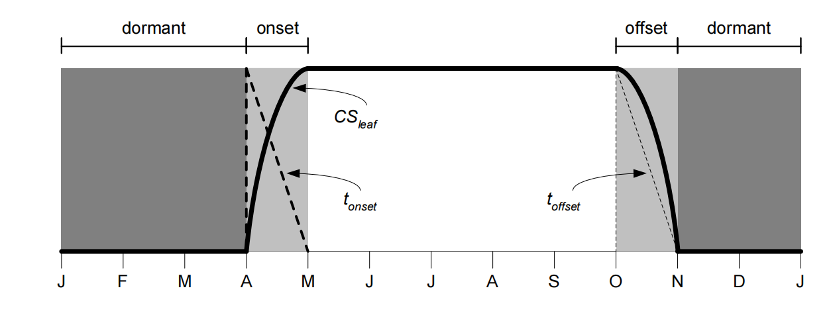
\includegraphics{Figures/植被生物地球化学循环过程/CoLM物候示意图.png}
\caption{CoLM物候示意图~\citep{lawrence2018}。 }
\label{fig:CoLM物候示意图}
\end{figure}
}

\item 活茎周转\\
CoLM物候模块中,在活茎的周转过程中,活茎细胞或活粗根最终死亡后变成死茎库或死粗根库的组成部分,
因此,活茎或活粗根碳每年固定比例($r_{lwt}$)进入死茎库或死粗根库:
\begin{equation}
CF_{ {livestem,deadstem }} = CS_{ {livestem }} r_{lwt}
\end{equation}
\begin{equation}
CF_{ {livecroot,deadcroot }} = CS_{ {livecroot }} r_{lwt}
\end{equation}
其中,$CF_{livestem,deadstem}$ 是活茎死亡变成死茎的碳通量,
$CF_{livecroot,deadcroot}$ 是活粗根死亡变成死粗根的碳通量。活茎和活粗根的周转时间是0.7年:
\begin{equation}
  \tau_{lwt} = \frac{0.7}{365 \cdot 86400}
\end{equation}
  对应的氮通量为:
\begin{equation}
NF_{livestem,deadstem} = CS_{livestem} r_{lwt} / CN_{dw}
\end{equation}
\begin{equation}
NF_{livecroot,deadcroot} = CS_{livecroot} r_{lwt} / CN_{dw}
\end{equation}
其中,$NF_{livestem,deadstem}$ 是活茎死亡变成死茎的氮,
$NF_{livecroot,deadcroot}$ 是活粗根死亡变成死粗根的氮,$CN_{dw}$ 是死茎和死粗根的碳氮比。

由于活茎和活粗根的碳氮比低于死茎和死粗根的碳氮比,所以从活茎或活粗根到死茎或死粗根的氮将会有一部分结余,存入植被再利用氮库:
\begin{equation}
NF_{{livestem,retrans}}=\left(\frac{CF_{{livestem,deadstem}}}{CN_{lw}}\right)-NF_{{livestem,deadstem}}
\end{equation}
\begin{equation}
NF_{{livecroot,retrans}}=\left(\frac{CF_{{livecroot,deadcroot}}}{CN_{lw}}\right)-NF_{{livecroot,deadcroot}}
\end{equation}
其中,$NF_{livestem,retrans}$ 是活茎死亡时回收再利用的氮,$NF_{livecroot,retrans}$ 是活粗根死亡时回收再利用的氮。

\end{enumerate}


\subsection{常绿植被的物候}\label{常绿植被的物候}
常绿植被功能型假设光合作用的净碳收入以及从土壤中的氮摄取直接分配给叶、细根、活茎和活粗茎的组织库。
代表非结构碳库的存储库和传输库将不会有任何碳存储。常绿植被功能型不存在特别的发芽展叶期和落叶期,
叶碳储量存在不随时间变化的固定碳周转速率:
\begin{equation}
\tau_{bglf}=\frac{1}{\tau_{leaf} \cdot 365 \cdot 86400}
\end{equation}
因此,叶面积指数的季节变化将主要由光合作用净碳收入的季节变化引起。
叶和细根的碳凋落通量($CF_{leaf,litter}$,$CF_{froot,litter}$)为:
\begin{equation}
CF_{leaf,litter}=r_{bglf} CS_{leaf}
\end{equation}
\begin{equation}
CF_{froot,litter}=r_{bglf} CS_{froot}
\end{equation}
相应的叶氮凋落通量($NF_{leaf,litter}$)、细根氮凋落通量($NF_{froot,litter}$)和再利用氮通量($NF_{leaf,retrans}$)为:
\begin{equation}
N F_{leaf,litter}=CS_{leaf,litter} / CN_{leaf_{litter}}
\end{equation}
\begin{equation}
N F_{froot,litter}=CS_{froot,litter} / CN_{froot}
\end{equation}
\begin{equation}
N F_{leaf,retrans}=\left(\frac{CF_{leaf,litter }}{CN_{leaf}}\right)-N F_{leaf,litter}
\end{equation}


\subsection{季节落叶植被的物候}\label{季节落叶植被的物候}
季节落叶植被功能型根据积温计算植被物候的发芽展叶期和落叶期,CoLM定义季节性落叶植被功能型仅存在于纬度大于19.5\textdegree 非赤道区域。
季节性落叶植被功能型假设植被每年仅存在一次发芽展叶期和落叶期。由于南北半球冬夏反季,
所以,通过白昼时长的变化判断冬季转变节点,积温($GDD$)的计算在冬季转变节点开始累积\citep{white1997continental}:
\begin{equation}
GDD _{sum}^{n}=\left\{\begin{array}{ll}GDD _{sum}^{n-1}+T_{s, 3} \cdot \Delta t \cdot 86400 & T_{s, 3} \geq \text{0 \textcelsius} \\ GDD _{sum}^{n-1} & T_{s, 3}< \text{0 \textcelsius}\end{array}\right.
\end{equation}
其中$GDD_{sum}^n$是第$n$天后的积温,积温通过对高于0 \textcelsius 的第三层土壤温度 $T_{s,3}$ (\textcelsius) 进行累加。
当$GDD_{sum}^n>{GDD}_{sum\_{crit}}$时,季节性落叶树开始发芽展叶期。${GDD}_{sum\_{crit}}$ 为发芽物候关键参量,
与前一年的温度 $T_{2m,ann\_{avg}}$ (\textcelsius)有关:
\begin{equation}
GDD _{sum\_{crit}}=\exp \left(4.8+0.13 \cdot T_{2 m, ann\_{avg}}\right)
\end{equation}
当发芽展叶期开始时,积温${GDD}_{sum}$重设为0,发芽展叶期倒计时重设:
\begin{equation}
t_{onset}=86400 \cdot n_{days\_on}
\end{equation}
其中$n_{days\_on}=30$,代表发芽展叶期倒计时30天。
同时,发芽展叶期开始的第一个时间步长 $\Delta t$ 内,50\% 的存储库中的碳进入传输库:
\begin{equation}
  CF_{leaf\_{stor},leaf\_{xfer}} = 0.5 CS_{leaf\_{stor}}/\Delta t
\end{equation}
\begin{equation}
  CF_{froot\_{stor},froot\_{xfer}} = 0.5  CS_{froot\_{stor}}/\Delta t
\end{equation}
\begin{equation}
  CF_{livestem\_{stor},livestem\_{xfer}} = 0.5  CS_{livestem\_{stor}}/\Delta t
\end{equation}
\begin{equation}
  CF_{deadstem\_{stor},deadstem\_{xfer}} = 0.5  CS_{deadstem\_{stor}}/\Delta t
\end{equation}
\begin{equation}
  CF_{livecroot\_{stor},livecroot\_{xfer}} = 0.5  CS_{livecroot\_{stor}}/\Delta t
\end{equation}
\begin{equation}
  CF_{deadcroot\_{stor},deadcroot\_{xfer}} = 0.5 CS_{deadcroot\_{stor}}/\Delta t
\end{equation}
\begin{equation}
  CF_{gresp\_{stor},gresp\_{xfer}} = 0.5  CS_{gresp\_{stor}}/\Delta t
\end{equation}
同时相应的氮传输:
\begin{equation}
NF_{leaf\_{stor},leaf\_{xfer}} = 0.5  NS_{leaf\_{stor}}/\Delta t
\end{equation}
%
\begin{equation}
  NF_{froot\_{stor},froot\_{xfer}} = 0.5  NS_{froot\_{stor}}/\Delta t
\end{equation}
%
\begin{equation}
  NF_{livestem\_{stor},livestem\_{xfer}} = 0.5  NS_{livestem\_{stor}}/\Delta t
\end{equation}
%
\begin{equation}
  NF_{deadstem\_{stor},deadstem\_{xfer}} = 0.5 NS_{deadstem\_{stor}}/\Delta t
\end{equation}
%
\begin{equation}
  NF_{livecroot\_{stor},livecroot\_{xfer}} = 0.5  NS_{livecroot\_{stor}}/\Delta t
\end{equation}
%
\begin{equation}
  NF_{deadcroot\_{stor},deadcroot\_{xfer}} = 0.5 NS_{deadcroot\_{stor}}/\Delta t
\end{equation}
%
\begin{equation}
  NF_{gresp\_{stor},gresp\_{xfer}} = 0.5 NS_{gresp\_{stor}}/\Delta t
\end{equation}


如果到夏天,日照长度缩短时还未开始发芽展叶期,
$GDD_{sum}^n$ 重设为0直至冬天。当发芽展叶期开始后,30天倒计时开始,直至 $t_{onset}=0$,发芽展叶期结束:
%
\begin{equation}
t_{onset}^n=t_{onset}^{n-1}-\Delta t
\end{equation}
当日照长度低于39300秒时,植被进入落叶期,落叶期倒计时为15天:
\begin{equation}
  t_{offset}^n=t_{offset}^{n-1}-\Delta t
\end{equation}


\subsection{胁迫落叶植被的物候}

胁迫落叶植被功能型包括草地和热带干旱落叶树等可以既响应干旱又响应温度胁迫。
当胁迫不存在时,该植被类型的物候还可以转变为常绿树的物候。当胁迫触发时,传输库的碳很快转变为组织库的碳。


当温度暖和,干旱成为触发胁迫的主要条件。当上一次落叶期结束后,土壤水分因子就开始从0累加:
\begin{equation}
SWI_{sum}^{n}=\left\{\begin{array}{ll}SWI_{sum}^{n-1}+f_{d a y} & \text{ 当 } \Psi_{s, 3} \geq-0.6\ \mathrm{MPa} \\ 
SWI_{sum}^{n} &  \text{ 当 } \Psi_{s, 3}<-0.6\ \mathrm{MPa}
\end{array}\right.
\end{equation}
其中$\Psi_{s,3}$是第三层土壤的水势,当土壤水势高于 -0.6 MPa 时,土壤足够湿润,土壤水分因子就开始累加。
当土壤水分因子高于15,同时过去十天有至少 20 mm 的降水,并且冷温胁迫没有触发,日照时长超过6小时,植被进入发芽展叶期。


同时,因为土壤温度过低 ($FD_{sum}^n>15$),需要应用冷气候标准
\begin{equation}
FD_{sum}^{n}=\left\{\begin{array}{ll}FD_{sum}^{n-1}+f_{day} &  \text{ 当 } T_{s, 3} > \text{0 \textcelsius} \\ 
FD_{sum}^{n-1} &  \text{ 当 } T_{s, 3} \leq \text{0 \textcelsius}
\end{array}\right.
\end{equation}
即当气温低,发芽展叶期的触发需要土壤温度和土壤湿度同时满足条件:
$SWI_{sum}>15,\ GDD_{sum}>GDD_{sum\_crit}$,和日照时长大于6小时。
当发芽展叶期开始后,30天倒计时开始,直至$t_{onset}=0$,发芽展叶期结束:
\begin{equation}
t_{o n s e t}^{n}=t_{o n s e t}^{n-1}-\Delta t
\end{equation}
当持续土壤干旱或持续低温或日照长度低于6小时,胁迫落叶期就将触发。
土壤干旱用累积落叶土壤水分因子($OSWI_{sum}^n$)来量化:
\begin{equation}
OSWI_{sum}^{n}=\left\{\begin{array}{ll}OSWI_{sum}^{n-1}+f_{d a y}, &  \text{ 当 } \Psi_{s, 3}<-2\ \mathrm{MPa} \\ 
\max \left(OSWI_{sum}^{n-1}-f_{d a y}, 0\right) &  \text{ 当 } \Psi_{s, 3}>-2\ \mathrm{MPa}
\end{array}\right.
\end{equation}
当前面一个发芽展叶期已经完成时,且$OSWI_{sum}^n\geq15$,即触发落叶期。
冷温胁迫用累积落叶冷冻天数来量化:
\begin{equation}
OFD_{sum}^{n}=\left\{\begin{array}{ll}OFD_{sum}^{n-1}+f_{d a y} &  \text{ 当 }{T}_{s, 3} \leq \text{0 \textcelsius} \\ 
\max \left(OFD_{sum}^{n-1}-f_{d a y}, 0\right) & \text{ 当 }{T}_{s, 3}> \text{0 \textcelsius}\end{array}\right.
\end{equation}
当前面一个发芽展叶期已经完成时,且$OFD_{sum}^n\geq15$,即触发落叶期。


总而言之,当以上三个条件($OSWI_{sum}^n\geq15$,$OFD_{sum}^n\geq15$,日照时长小于6小时)满足其一,植被进入落叶期,落叶期倒计时为15天:
\begin{equation}
t_{offset}^{n}=t_{offset}^{n-1}-\Delta t
\end{equation}
当落叶条件始终不满足(1年以上),胁迫落叶植被功能型就表现为常绿物候。
长生长季控制变量($LGS$)被用来刻画该常绿物候的周转速率:
\begin{equation}
\tau_{b g l f}=\frac{L G S}{\tau_{leaf} \cdot 365 \cdot 86400}
\end{equation}

\begin{equation}
L G S=\left\{\begin{array}{cc}0 &  \text{ 当 } n_{ {days}\_{active}}<365 \\ 
\frac{n_{ {days\_{active}}}}{365}-1 &  \text{ 当 } 365 \leq n_{ {days }\_{active} }<730 \\ 
1 & \text{ 当 } n_{ {days}\_{active}} \geq 730
\end{array}\right.
\end{equation}
$n_{days\_{active}}$ 是植被只从上次发芽开始的天数。


每个时间步长,都有储存库的碳进入传输库:
\begin{equation}
CF_{leaf\_{stor},leaf\_{xfer}}=CS_{leaf\_{stor} } \tau_{bgtr}
\end{equation}
\begin{equation}
CF_{ {froot }\_{stor},{ froot }\_{xfer }}=CS_{{froot }\_{stor}} \tau_{bgtr}
\end{equation}
\begin{equation}
 CF_{livestem\_{stor},livestem\_{xfer}}=CS_{livestem\_{stor}}\tau_{bgtr}
\end{equation}
\begin{equation}
 CF_{deadstem\_{stor},deadstem\_{xfer}}=CS_{deadstem\_{stor}}\tau_{bgtr}
\end{equation}
\begin{equation}
  CF_{livecroot\_{stor},livecroot\_{xfer}}=CS_{livecroot\_{stor}}\tau_{bgtr}
\end{equation}
\begin{equation}
  CF_{deadcroot\_{stor},deadcroot\_{xfer}}=CS_{deadcroot\_{stor}}\tau_{bgtr}
\end{equation}
传输库碳全部进入组织库:
\begin{equation}
  CF_{leaf\_{xfer},leaf}=CS_{leaf\_{xfer}}/\Delta t
\end{equation}
\begin{equation}
  CF_{froot\_{xfer},froot}=CS_{froot\_{xfer}}/\Delta t
\end{equation}
\begin{equation}
  CF_{livestem\_{xfer},livestem}=CS_{livestem\_{xfer}}/\Delta t
\end{equation}
\begin{equation}
  CF_{deadstem\_{xfer},deadstem}=CS_{deadstem\_{xfer}}/\Delta t
\end{equation}
\begin{equation}
  CF_{livecroot\_{xfer},livecroot}=CS_{livecroot\_{xfer}}/\Delta t
\end{equation}
\begin{equation}
  CF_{deadcroot\_{xfer},deadcroot}=CS_{deadcroot\_{xfer}}/\Delta t
\end{equation}
对应的氮凋落物:
\begin{equation}
  NF_{leaf\_{stor},leaf\_{xfer}}=NS_{leaf\_{stor}}\tau_{bgtr}
\end{equation}
\begin{equation}
  NF_{froot\_{stor},froot\_{xfer}}=NS_{froot\_{stor}}\tau_{bgtr}
\end{equation}
\begin{equation}
  NF_{livestem\_{stor},livestem\_{xfer}}=NS_{livestem\_{stor}}\tau_{bgtr}
\end{equation}
\begin{equation}
  NF_{deadstem\_{stor},deadstem\_{xfer}}=NS_{deadstem\_{stor}}\tau_{bgtr}
\end{equation}
\begin{equation}
  NF_{livecroot\_{stor},livecroot\_{xfer}}=NS_{livecroot\_{stor}}\tau_{bgtr}
\end{equation}
\begin{equation}
  NF_{deadcroot\_{stor},deadcroot\_{xfer}}=NS_{deadcroot\_{stor}}\tau_{bgtr}
\end{equation}
传输库氮全部进入组织库:
\begin{equation}
  NF_{leaf\_{xfer},leaf}=NS_{leaf\_{xfer}}/\Delta t
\end{equation}
\begin{equation}
  NF_{froot\_{xfer},froot}=NS_{froot\_{xfer}}/\Delta t
\end{equation}
\begin{equation}
  NF_{livestem\_{xfer},livestem}=NS_{livestem\_{xfer}}/\Delta t
\end{equation}
\begin{equation}
  NF_{deadstem\_{xfer},deadstem}=NS_{deadstem\_{xfer}}/\Delta t
\end{equation}
\begin{equation}
  NF_{livecroot\_{xfer},livecroot}=NS_{livecroot\_{xfer}}/\Delta t
\end{equation}
\begin{equation}
  NF_{deadcroot\_{xfer},deadcroot}=NS_{deadcroot\_{xfer}}/\Delta t
\end{equation}


\subsection{物候凋落物}\label{物候凋落物}
物候的凋落物包括叶和细根,其中叶凋落物将进入代谢凋落物、
纤维素凋落物和木质部凋落物,细根凋落物同样进入代谢凋落物、纤维素凋落物和木质部凋落物:
\begin{equation}
  CF_{leaf,lit1}=\sum_{p}^{npft}{CF_{leaf,litter}f_{lab\_{leaf},p}{wcol_p}}
\end{equation}
\begin{equation}
  CF_{leaf,lit2}=\sum_{p}^{npft}{CF_{leaf,litter}f_{cel\_{leaf},p}{wcol_p}}
\end{equation}
\begin{equation}
  CF_{leaf,lit3}=\sum_{p}^{npft}{CF_{leaf,litter}f_{lig\_{leaf},p}{wcol_p}}
\end{equation}
\begin{equation}
  CF_{froot,lit1}=\sum_{p}^{npft}{CF_{froot,litter}f_{lab\_{froot},p}{wcol_p}}
\end{equation}
\begin{equation}
  CF_{froot,lit2}=\sum_{p}^{npft}{CF_{froot,litter}f_{cel\_{froot},p}{wcol_p}}
\end{equation}
\begin{equation}
  CF_{froot,lit3}=\sum_{p}^{npft}{CF_{froot,litter}f_{lig\_{froot},p}{wcol_p}}
\end{equation}
其中$f_{lab\_{leaf},p}$, $f_{cel\_{leaf},p}$ 和 $f_{lig\_{leaf},p}$ 是叶片凋落物中,
活性凋落物,纤维素和木质素凋落物占得比例,$f_{lab\_{leaf},p}$, $f_{cel\_{leaf},p}$
和 $f_{lig\_{leaf},p}$ 是细根凋落物中,活性凋落物,
纤维素和木质素凋落物占的比例,${wcol_p}$ 代表每个 patch 的面积比。

对应的氮通量可表达为:
\begin{equation}
  NF_{leaf,lit1}=\sum_{p}^{npft}{NF_{leaf,litter}f_{lab\_{leaf},p}{wcol_p}}
\end{equation}
\begin{equation}
  NF_{leaf,lit2}=\sum_{p}^{npft}{NF_{leaf,litter}f_{cel\_{leaf},p}{wcol_p}}
\end{equation}
\begin{equation}
  NF_{leaf,lit3}=\sum_{p}^{npft}{NF_{leaf,litter}f_{lig\_{leaf},p}{wcol_p}}
\end{equation}
\begin{equation}
  NF_{froot,lit1}=\sum_{p}^{npft}{NF_{froot,litter}f_{lab\_{froot},p}{wcol_p}}
\end{equation}
\begin{equation}
  NF_{froot,lit2}=\sum_{p}^{npft}{NF_{froot,litter}f_{cel\_{froot},p}{wcol_p}}
\end{equation}
\begin{equation}
  NF_{froot,lit3}=\sum_{p}^{npft}{NF_{froot,litter}f_{lig\_{froot},p}{wcol_p}}
\end{equation}


\subsection{植被的自然死亡}\label{植被的自然死亡}
植被的整体自然死亡率被假设为2\%每年。
所有的叶、细根、活茎、死茎、或粗根和死粗根的组织库、存储库和传输库受死亡率的控制,
其凋落物碳氮通量为: 


\begin{equation}
  CF_{leaf\_{mort}}=CS_{leaf}\cdot \frac{0.2\%}{365\cdot 86400}
\end{equation}
\begin{equation}
  CF_{froot\_mort}=CS_{froot}\cdot \frac{0.2\%}{365\cdot 86400}
\end{equation}
\begin{equation}
  CF_{livestem\_mort}=CS_{livestem}\cdot \frac{0.2\%}{365\cdot 86400}
\end{equation}
\begin{equation}
  CF_{deadstem\_mort}=CS_{deadstem}\cdot \frac{0.2\%}{365\cdot 86400}
\end{equation}
\begin{equation}
  CF_{livecroot\_mort}=CS_{livecroot}\cdot \frac{0.2\%}{365\cdot 86400}
\end{equation}
\begin{equation}
  CF_{deadcroot\_mort}=CS_{deadcroot}\cdot \frac{0.2\%}{365\cdot 86400}
\end{equation}
\begin{equation}
  NF_{leaf\_{mort}}=NS_{leaf}\cdot \frac{0.2\%}{365\cdot 86400}
\end{equation}
\begin{equation}
  NF_{froot\_mort}=NS_{froot}\cdot \frac{0.2\%}{365\cdot 86400}
\end{equation}
\begin{equation}
  NF_{livestem\_mort}=NS_{livestem}\cdot \frac{0.2\%}{365\cdot 86400}
\end{equation}
\begin{equation}
  NF_{deadstem\_mort}=NS_{deadstem}\cdot \frac{0.2\%}{365\cdot 86400}
\end{equation}
\begin{equation}
  NF_{livecroot\_mort}=NS_{livecroot}\cdot \frac{0.2\%}{365\cdot 86400}
\end{equation}
\begin{equation}
  NF_{deadcroot\_mort}=NS_{deadcroot}\cdot \frac{0.2\%}{365\cdot 86400}
\end{equation}
存储库的凋落:
\begin{equation}
  CF_{leaf\_{{stor}\_{mort}}}=CS_{leaf\_{stor}}\cdot \frac{0.2\%}{365\cdot 86400}
\end{equation}
\begin{equation}
  CF_{froot\_{{stor}\_{mort}}}=CS_{froot\_{stor}}\cdot \frac{0.2\%}{365\cdot 86400}
\end{equation}
\begin{equation}
CF_{livestem\_{{stor}\_{mort}}}=CS_{livestem\_{stor}}\cdot \frac{0.2\%}{365\cdot 86400}
\end{equation}
\begin{equation}
  CF_{deadstem\_{{stor}\_{mort}}}=CS_{deadstem\_{stor}}\cdot \frac{0.2\%}{365\cdot 86400}
\end{equation}
\begin{equation}
  CF_{livecroot\_{{stor}\_{mort}}}=CS_{livecroot\_{stor}}\cdot \frac{0.2\%}{365\cdot 86400}
\end{equation}
\begin{equation}
  CF_{deadcroot\_{{stor}\_{mort}}}=CS_{deadcroot\_{stor}}\cdot \frac{0.2\%}{365\cdot 86400}
\end{equation}
\begin{equation}
  NF_{leaf\_{{stor}\_{mort}}}=NS_{leaf\_{stor}}\cdot \frac{0.2\%}{365\cdot 86400}
\end{equation}
\begin{equation}
  NF_{froot\_{{stor}\_{mort}}}=NS_{froot\_{stor}}\cdot \frac{0.2\%}{365\cdot 86400}
\end{equation}
\begin{equation}
  NF_{livestem\_{{stor}\_{mort}}}=NS_{livestem\_{stor}}\cdot \frac{0.2\%}{365\cdot 86400}
\end{equation}
\begin{equation}
  NF_{deadstem\_{{stor}\_{mort}}}=NS_{deadstem\_{stor}}\cdot \frac{0.2\%}{365\cdot 86400}
\end{equation}
\begin{equation}
  NF_{livecroot\_{{stor}\_{mort}}}=NS_{livecroot\_{stor}}\cdot \frac{0.2\%}{365\cdot 86400}
\end{equation}
\begin{equation}
  NF_{deadcroot\_{{stor}\_{mort}}}=NS_{deadcroot\_{stor}}\cdot \frac{0.2\%}{365\cdot 86400}
\end{equation}
\begin{equation}
  CF_{leaf\_{{xfer}\_{mort}}}=CS_{leaf\_{xfer}}\cdot \frac{0.2\%}{365\cdot 86400}
\end{equation}
\begin{equation}
  CF_{froot\_{{xfer}\_{mort}}}=CS_{froot\_{xfer}}\cdot \frac{0.2\%}{365\cdot 86400}
\end{equation}
\begin{equation}
  CF_{livestem\_{{xfer}\_{mort}}}=CS_{livestem\_{xfer}}\cdot \frac{0.2\%}{365\cdot 86400}
\end{equation}
\begin{equation}
  CF_{deadstem\_{{xfer}\_{mort}}}=CS_{deadstem\_{xfer}}\cdot \frac{0.2\%}{365\cdot 86400}
\end{equation}
\begin{equation}
  CF_{livecroot\_{{xfer}\_{mort}}}=CS_{livecroot\_{xfer}}\cdot \frac{0.2\%}{365\cdot 86400}
\end{equation}
\begin{equation}
  CF_{deadcroot\_{{xfer}\_{mort}}}=CS_{deadcroot\_{xfer}}\cdot \frac{0.2\%}{365\cdot 86400}
\end{equation}
\begin{equation}
  NF_{leaf\_{{xfer}\_{mort}}}=NS_{leaf\_{xfer}}\cdot \frac{0.2\%}{365\cdot 86400}
\end{equation}
\begin{equation}
  NF_{froot\_{{xfer}\_{mort}}}=NS_{froot\_{xfer}}\cdot \frac{0.2\%}{365\cdot 86400}
\end{equation}
\begin{equation}
  NF_{livestem\_{{xfer}\_{mort}}}=NS_{livestem\_{xfer}}\cdot \frac{0.2\%}{365\cdot 86400}
\end{equation}
\begin{equation}
  NF_{deadstem\_{{xfer}\_{mort}}}=NS_{deadstem\_{xfer}}\cdot \frac{0.2\%}{365\cdot 86400}
\end{equation}
\begin{equation}
  NF_{livecroot\_{{stor}\_{mort}}}=NS_{livecroot\_{stor}}\cdot \frac{0.2\%}{365\cdot 86400}
\end{equation}
\begin{equation}
  NF_{deadcroot\_{{stor}\_{mort}}}=NS_{deadcroot\_{stor}}\cdot \frac{0.2\%}{365\cdot 86400}
\end{equation}
死亡的植被碳氮通量将进入凋落物库:
\begin{equation}
CF_{leaf\_{mort},lit1}=\sum_{p=0}^{npft}{CF_{leaf\_{mort}}f_{lab\_{leaf},p}{wcol_p}}
\end{equation}
\begin{equation}
CF_{leaf\_{mort},lit2}=\sum_{p=0}^{npft}{CF_{leaf\_{mort}}f_{cel\_{leaf},p}{wcol_p}}
\end{equation}
\begin{equation}
CF_{leaf\_{mort},lit3}=\sum_{p=0}^{npft}{CF_{leaf\_{mort}}f_{lig\_{leaf},p}{wcol_p}}
\end{equation}
\begin{equation}
CF_{froot\_mort,lit1}=\sum_{p=0}^{npft}{CF_{froot\_mort}f_{lab\_{leaf},p}{wcol_p}}
\end{equation}
\begin{equation}
CF_{froot\_mort,lit2}=\sum_{p=0}^{npft}{CF_{froot\_mort}f_{cel\_{leaf},p}{wcol_p}}
\end{equation}
\begin{equation}
CF_{froot\_mort,lit3}=\sum_{p=0}^{npft}{CF_{froot\_mort}f_{lig\_{leaf},p}{wcol_p}}
\end{equation}
\begin{equation}
NF_{leaf\_{mort},lit1}=\sum_{p=0}^{npft}{NF_{leaf\_{mort}}f_{lab\_{leaf},p}{wcol_p}}
\end{equation}
\begin{equation}
  NF_{leaf\_{mort},lit2}=\sum_{p=0}^{npft}{NF_{leaf\_{mort}}f_{cel\_{leaf},p}{wcol_p}}
\end{equation}
\begin{equation}
  NF_{leaf\_{mort},lit3}=\sum_{p=0}^{npft}{NF_{leaf\_{mort}}f_{lig\_{leaf},p}{wcol_p}}
\end{equation}
\begin{equation}
  NF_{froot\_mort,lit1}=\sum_{p=0}^{npft}{NF_{froot\_mort}f_{lab\_{leaf},p}{wcol_p}}
\end{equation}
\begin{equation}
  NF_{froot\_mort,lit2}=\sum_{p=0}^{npft}{NF_{froot\_mort}f_{cel\_{leaf},p}{wcol_p}}
\end{equation}
\begin{equation}
  NF_{froot\_mort,lit3}=\sum_{p=0}^{npft}{NF_{froot\_mort}f_{lig\_{leaf},p}{wcol_p}}
\end{equation}
其中$f_{lab\_{leaf},p}$, $f_{cel\_{leaf},p}$ 和 $f_{lig\_{leaf},p}$ 是叶片凋落物中,
活性凋落物,纤维素和木质素凋落物占得比例,$f_{lab\_{leaf},p}$, $f_{cel\_{leaf},p}$ 和 $f_{lig\_leaf,p}$
是细根凋落物中,活性凋落物,纤维素和木质素凋落物占的比例,${wcol_p}$ 代表每个 patch 的面积比。


活茎、死茎、活粗根和死粗根在树木死亡后进入木质部残体库:
\begin{equation}
  CF_{livestem\_{mort},cwd}=\sum_{p=0}^{npft}{CF_{livestem\_{mort}}{wcol_p}}
\end{equation}
\begin{equation}
  CF_{deadstem\_{mort},cwd}=\sum_{p=0}^{npft}{CF_{deadstem\_{mort}}{wcol_p}}
\end{equation}
\begin{equation}
  CF_{livecroot\_{mort},cwd}=\sum_{p=0}^{npft}{CF_{livecroot\_{mort}}{wcol_p}}
\end{equation}
\begin{equation}
  CF_{deadcroot\_{mort},cwd}=\sum_{p=0}^{npft}{CF_{deadcroot\_{mort}}{wcol_p}}
\end{equation}
\begin{equation}
  NF_{livestem\_{mort},cwd}=\sum_{p=0}^{npft}{NF_{livestem\_{mort}}{wcol_p}}
\end{equation}
\begin{equation}
  NF_{deadstem\_{mort},cwd}=\sum_{p=0}^{npft}{NF_{deadstem\_{mort}}{wcol_p}}
\end{equation}
\begin{equation}
  NF_{livecroot\_{mort},cwd}=\sum_{p=0}^{npft}{NF_{livecroot\_{mort}}{wcol_p}}
\end{equation}
\begin{equation}
  NF_{deadcroot\_{mort},cwd}=\sum_{p=0}^{npft}{NF_{deadcroot\_{mort}}{wcol_p}}
\end{equation}
此外,所有的含有非结构碳氮的储存库和传输库在植被死亡后都进入代谢凋落物库中:
\begin{equation}
  CF_{leaf\_{{stor}\_{mort}},lit1}=\sum_{p=0}^{npft}{CF_{leaf\_{{stor}\_{mort}}}{wcol_p}}
\end{equation}
\begin{equation}
  CF_{froot\_{{stor}\_{mort}},lit1}=\sum_{p=0}^{npft}{CF_{froot\_{{stor}\_{mort}}}{wcol_p}}
\end{equation}
\begin{equation}
  CF_{livestem\_{{stor}\_{mort}},lit1}=\sum_{p=0}^{npft}{CF_{livestem\_{{stor}\_{mort}}}{wcol_p}}
\end{equation}
\begin{equation}
  CF_{deadstem\_{{stor}\_{mort}},lit1}=\sum_{p=0}^{npft}{CF_{deadstem\_{{stor}\_{mort}}}{wcol_p}}
\end{equation}
\begin{equation}
  CF_{livecroot\_{{stor}\_{mort}},lit1}=\sum_{p=0}^{npft}{CF_{livecroot\_{{stor}\_{mort}}}{wcol_p}}
\end{equation}
\begin{equation}
  CF_{deadcroot\_{{stor}\_{mort}},lit1}=\sum_{p=0}^{npft}{CF_{deadcroot\_{{stor}\_{mort}}}{wcol_p}}
\end{equation}
\begin{equation}
  CF_{gresp\_{{stor}\_{mort}},lit1}=\sum_{p=0}^{npft}{CF_{gresp\_{{stor\_{mort}}}}{wcol_p}}
\end{equation}
\begin{equation}
  CF_{leaf\_{xfer\_{mort,lit1}}}=\sum_{p=0}^{npft}{CF_{leaf\_{{xfer\_{mort}}}}{wcol_p}}
\end{equation}
\begin{equation}
  CF_{froot\_{xfer\_{mort,lit1}}}=\sum_{p=0}^{npft}{CF_{froot\_{{xfer\_{mort}}}}{wcol_p}}
\end{equation}
\begin{equation}
  CF_{livestem\_{xfer\_{mort,lit1}}}=\sum_{p=0}^{npft}{CF_{livestem\_{{xfer\_{mort}}}}{wcol_p}}
\end{equation}
\begin{equation}
  CF_{deadstem\_{xfer\_{mort,lit1}}}=\sum_{p=0}^{npft}{CF_{deadstem\_{xfer\_{mort}}}{wcol_p}}
\end{equation}
\begin{equation}
  CF_{livecroot\_{xfer\_{mort,lit1}}}=\sum_{p=0}^{npft}{CF_{livecroot\_{{xfer\_{mort}}}}{wcol_p}}
\end{equation}
\begin{equation}
  CF_{deadcroot\_{xfer\_{mort,lit1}}}=\sum_{p=0}^{npft}{CF_{deadcroot\_{{xfer\_{mort}}}}{wcol_p}}
\end{equation}
\begin{equation}
  CF_{gresp\_{xfer\_{mort,lit1}}}=\sum_{p=0}^{npft}{CF_{gresp\_{{xfer}\_{mort}}}{wcol_p}}
\end{equation}
对应的氮通量中,植被死亡后,再利用氮库进入代谢凋落物库:
\begin{equation}
  NF_{leaf\_{{stor}\_{mort}},lit1}=\sum_{p=0}^{npft}{NF_{leaf\_{{stor}\_{mort}}}{wcol_p}}
\end{equation}
\begin{equation}
  NF_{froot\_{{stor}\_{mort}},lit1}=\sum_{p=0}^{npft}{NF_{froot\_{{stor}\_{mort}}}{wcol_p}}
\end{equation}
\begin{equation}
  NF_{livestem\_{{stor}\_{mort}},lit1}=\sum_{p=0}^{npft}{NF_{livestem\_{{stor}\_{mort}}}{wcol_p}}
\end{equation}
\begin{equation}
  NF_{deadstem\_{{stor}\_{mort}},lit1}=\sum_{p=0}^{npft}{NF_{deadstem\_{{stor}\_{mort}}}{wcol_p}}
\end{equation}
\begin{equation}
  NF_{retrans\_{mort,lit1}}=\sum_{p=0}^{npft}{NF_{retrans\_{mort}}{wcol_p}}
\end{equation}
\begin{equation}
  NF_{leaf\_{{xfer}\_{mort,lit1}}}=\sum_{p=0}^{npft}{NF_{{leaf}\_{xfer\_{mort}}}{wcol_p}}
\end{equation}
\begin{equation}
  NF_{froot\_{xfer\_{mort,lit1}}}=\sum_{p=0}^{npft}{NF_{froot\_{xfer\_{mort}}}}{wcol_p}
\end{equation}
\begin{equation}
  NF_{livestem\_{xfer\_{mort,lit1}}}=\sum_{p=0}^{npft}{NF_{livestem\_{xfer\_{mort}}}{wcol_p}}
\end{equation}
\begin{equation}
NF_{deadstem\_{xfer\_{mort,lit1}}}=\sum_{p=0}^{npft}{NF_{deadstem\_{xfer\_{mort}}}{wcol_p}}
\end{equation}
\begin{equation}
  NF_{livecroot\_{xfer\_{mort,lit1}}}=\sum_{p=0}^{npft}{NF_{livecroot\_{xfer\_{mort}}}{wcol_p}}
\end{equation}
\begin{equation}
  NF_{deadcroot\_{xfer\_{mort,lit1}}}=\sum_{p=0}^{npft}{NF_{deadcroot\_{xfer\_{mort}}}{wcol_p}}
\end{equation}

